\newpage
\section{基础术语与模型评估}

\subsection{基本术语}
\subsubsection{数据}
输入 $\to$ 输出. 

机械学习是面向输出的技术. 

术语扩展:
\begin{itemize}
    \item 特征 (属性)
    \item 属性值: 离散或连续
    \item 样本维度: 特征个数
    \item 特征张成的空间 (属性空间/特征空间/输入空间)
    \item 标记张成的空间 (标记空间/输出空间)
    \item 示例/样本: 一个对象的输入 (不含标记)
    \item 样例: 示例+标记
    \item 训练集: 一组训练样例
    \item 测试集: 一组测试样例
\end{itemize}

\subsubsection{任务}
\paragraph{预测任务}: 根据标记取值的情况
\begin{itemize}
    \item 分类任务: 标记为离散值
    \subitem 二分类
    \subitem 多分类
    \item 回归任务: 标记为连续值
    \item 聚类任务: 标记为空值, 对示例进行分组
\end{itemize}
根据标记完整性的情况
\begin{itemize}
    \item 监督学习: 所有示例有标记
    \subitem e.g. 分类, 回归
    \item 无监督学习: 所有示例无标记
    \subitem e.g. 聚类
    \item 半监督学习: 少量示例有标记, 大量示例无标记
\end{itemize}

\subsubsection{目标}
泛化能力: 应对未来未见测试样本的能力. 

I.I.D (独立同分布)假设: 历史与未来来自相同分布

\subsection{概念学习}
最理想的机器学习技术是学习到 概念 (语言的边界就是思维的边界)
\subsubsection{假设空间}
假设空间: 枚举所有可能的假设

版本空间(假设空间的子集): 跟训练集一致的``假设集合''. 

\subsubsection{归纳偏好}
Inductive bias: 学习过程中对某种类型假设的偏好称作归纳偏好

\begin{theorem}[No Free Lunch]
    一个算法 $\zeta_a$ 如果在某些问题上比另一个算法 $\zeta_b$ 好, 必然存在另一些问题, $\zeta_b$ 比 $\zeta_a$ 好.
\end{theorem}
因为未来数据是不知道的,总有一种未来数据的分布让你失败
\begin{proof}
    假设样本空间 $\mathcal{X}$ 和假设空间 $\mathcal{H}$ 都是离散的. 令 $P(h|X, \mathfrak{L}_a)$ 代表算法 $\mathfrak{L}_a$ 基于训练数据 $X$ 产生假设 $h$ 的概率, 再令 $f$ 代表我们希望学习的真实目标函数. $\mathfrak{L}_a$ 的 ``训练集外误差'', 即 $\mathfrak{L}_a$ 在训练集之外的所有样本上的误差为
    \begin{align*}
        E_{ote}(\mathfrak{L}_a|X, f)=\sum_h\sum_{\bm{x}\in \mathcal{X}-X}P(\bm{x}) \mathbb{I} (h(\bm x) \ne f (\bm x ))P(h|X,\mathfrak{L}_a)
    \end{align*}
    其中 $\mathbb{I}(\cdot)=\left\{ \begin{array}{ll}
        1 & \cdot\text{ is true}\\0 & \text{otherwise}
    \end{array} \right.$ 为指示函数.

    以二分类问题为例, $\forall f: \mathcal{X} \mapsto \{0,1\}$, 函数空间 (所有可能映射的数量)为 $\{0,1\}^{|\mathcal{X}|}$. 对所有 $f$ 求和, 有
    \begin{align*}
        &\sum_f E_{ote}(\mathfrak{L}_a|X, f)\\
        =&\sum_f \sum_h\sum_{\bm{x}\in \mathcal{X}-X}P(\bm{x}) \mathbb{I} (h(\bm x) \ne f (\bm x ))P(h|X,\mathfrak{L}_a)\\
        =&\sum_{\bm{x}\in \mathcal{X}-X}P(\bm x)\sum_h P(h|X,\mathfrak{L}_a)\sum_f \mathbb{I}(h(\bm x) \ne f (\bm x ))\\
        =&\sum_{\bm{x}\in \mathcal{X}-X}P(\bm x)\sum_h P(h|X,\mathfrak{L}_a)\frac{1}{2}2^{|\mathcal{X}|}\\
        =&\frac{1}{2}2^{|\mathcal{X}|}\sum_{\bm{x}\in \mathcal{X}-X}P(\bm x)\sum_h P(h|X,\mathfrak{L}_a)\\
        =&2^{|\mathcal{X}|-1}\sum_{\bm{x}\in \mathcal{X}-X}P(\bm x) 
    \end{align*}
    $\forall \mathfrak{L}_a, \mathfrak{L}_b$, 有
    \begin{align*}
        \sum_f E_{ote}(\mathfrak{L}_a|X, f)=\sum_f E_{ote}(\mathfrak{L}_b|X, f)
    \end{align*} 
    即不同学习算法的性能期望一致 (严谨证明更加复杂)
\end{proof}

若 $f$ 均 匀 分 布 ,则有一半 的 $f$ 对 $\bm{x}$ 的预测与 $h(x)$ 不一致. 所以 $\sum_f \mathbb{I}(h(\bm x) \ne f (\bm x ))=\frac{1}{2}2^{|\mathcal{X}|}$

证明了总误差与学习算法无关. 

\subsection{模型评估与选择}

\subsubsection{经验误差与过拟合}
经验误差: 
\begin{itemize}
    \item 错误率 error rate: 错分样本的占比 $E=\frac{a}{m}$
    \item 误差 error: 样本真实输出与预测输出之间的差异
    \subitem 训练误差: 训练集的误差
    \subitem 测试误差: 测试集的误差
\end{itemize}

拟合:
\begin{itemize}
    \item 过拟合: 将训练样本本身的特点, 当作所有样本的一般性质. 
    \item 欠拟合: 对训练样本的一般性质尚未学好
\end{itemize}

\subsubsection{评估方法}
\begin{itemize}
    \item 留出法(hold-out): 分为两个互斥集合
    \item 交叉验证法 (cross-validation): 分为 $k$ 个子集, 轮流当测试集. 
    \item 自助法 (bootstrapping): 以一个概率采样样本, 允许重复, 适用于小数据. 
    \item 在验证集上调参
\end{itemize}


\subsubsection{性能度量}
性能度量衡量泛化能力. 

对于回归任务, 度量最常用的是均方误差:
\begin{align*}
    E(f;D)=\frac{1}{m}\sum_{i=1}^mf((x_i)-y_i)^2
\end{align*}


对于分类任务:
\begin{itemize}
    \item 错误率: 分错样本占总样本数的比例
    \item 精度: 分对样本占总样本数的比例
\end{itemize}
错误率+精度=1

\paragraph{混淆矩阵}\quad

\begin{table}[!htb]
    \centering
    \caption{混淆矩阵}
    \begin{tabular}[c]{|r|c|c|}\hline
        & Relevant & Irrelevant\\ \hline
        Retrieved & $R_R$ & $I_R$\\ \hline
        Not Retrieved & $R_N$ & $I_N$ \\  \hline
    \end{tabular}
\end{table}
\begin{align*}
    \text{Precision(查准率) }P&=\frac{R_R}{R_R+I_R}\\
    \text{Recall(查全率) }R&=\frac{R_R}{R_R+R_N}
\end{align*}

\paragraph{P-R 曲线}查准率-查全率曲线, 平衡点: Precision$=$Recall. 
\begin{figure}[H]
    \centering
    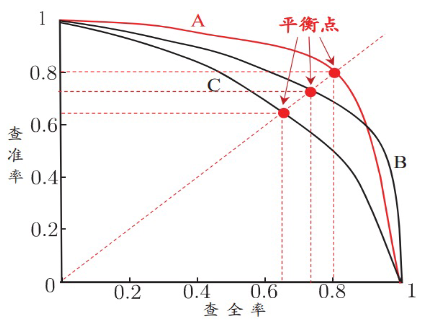
\includegraphics[width=0.309\textwidth]{pic/ML2/P-R 曲线 与平衡点.png}
    \caption{P-R 曲线 与平衡点}
\end{figure}

\paragraph{\texorpdfstring{$F_\beta$}. 度量} 更常用
\begin{align*}
    F_\beta=\frac{(1+\beta)^2\times P \times R}{(\beta^2 \times P)+R}
\end{align*}
\begin{itemize}
    \item $\beta=1$: 标准 $F_1$
    \item $\beta>1$: 偏重 Recall
    \item $\beta<1$: 偏重 Precision
\end{itemize}

其来自对 $P$, $R$ 的加权调和平均:
\begin{align*}
    \frac{1}{F_\beta}=\frac{1}{1+\beta^2}\left( \frac{1}{P}+\frac{\beta^2}{R} \right)
\end{align*}

\paragraph{ROC 与 AUC}ROC 全称受试者工作特征(Receiver Operating Characteristic)曲线. AUC 值: 衡量样本预测的排序质量. 

\begin{figure}[!htb]
    \centering
    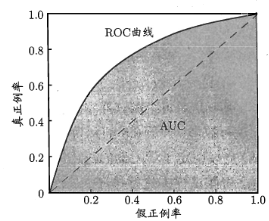
\includegraphics[width=0.309\textwidth]{pic/ML2/ROC曲线与AUC.png}
    \caption{ROC曲线与AUC}
\end{figure}


\paragraph{代价敏感错误率}为 错 误 赋 予 ``非均等代价''(unequal cost).



\subsubsection{比较检验}%TODO 
\paragraph{二项检验}


\paragraph{T-检验}

\paragraph{交叉验证 T-检验}



\subsubsection{偏差与方差}
偏差-方差分解帮助解释泛化性能. 

对测试样本 $\bx$, 令 $y_D$ 为 $\bx$ 在数据集中的标记, $y$ 为 $\bx$ 的真实标记, $f(\bx;D)$ 为训练集 $D$ 上学得模型$f$在$\bx$上的预测输出. 以回归任务为例, 学习算法的期望预测为
\begin{align*}
    \bar{f}(\bx)=\mathbb{E}_D\left[ f(\bx;D) \right]
\end{align*}
使用样本数相同的不同训练集产生的方差为
\begin{align*}
    var(\bx)=\mathbb{E}_D\left[ \left( f(\bx;D)-\bar{f}(\bx) \right)^2 \right]
\end{align*}
噪声为
\begin{align*}
    \epsilon^2=\mathbb{E}\left[ (y_D-y)^2 \right]
\end{align*}
期望输出与真实标记的差别称为偏差(bias),即
\begin{align*}
    bias^2(\bx)=\left( \bar{f}(\bx)-y \right)^2
\end{align*}

为便于讨论,假定噪声期望为零,即 $\mathbb{E}_D[y_D-y]=0$ . 通过简单的多项式展开合并,可对算法的期望泛化误差进行分解:
\begin{align*}
    E(f;D)=& \mathbb{E}_D\left[ \left( f(\bx;D)-y_D \right)^2 \right]\\
    =& \mathbb{E}_D\left[ \left( f(\bx;D)-\bar{f}(\bx)+\bar{f}(\bx)-y_D \right)^2 \right]\\
    =& \mathbb{E}_D\left[ \left( f(\bx;D)-\bar{f}(\bx) \right)^2 \right] + \mathbb{E}_D\left[ \left(\bar{f}(\bx)-y_D \right)^2 \right]\\
    &+\mathbb{E}_D\left[ 2\left( f(\bx;D)-\bar{f}(\bx)\right)\left(\bar{f}(\bx)-y_D \right) \right]\\
    =&\mathbb{E}_D\left[ \left( f(\bx;D)-\bar{f}(\bx) \right)^2 \right]\\
    & + \mathbb{E}_D\left[ \left(\bar{f}(\bx)-y+y-y_D \right)^2 \right]\\
    =&\mathbb{E}_D\left[ \left( f(\bx;D)-\bar{f}(\bx) \right)^2 \right]\\
    & + \mathbb{E}_D\left[ \left(\bar{f}(\bx)-y\right)^2 \right]+\mathbb{E}_D\left[ \left(y-y_D \right)^2 \right]\\
    &+\mathbb{E}_D\left[ 2\left( \bar{f} (\bx) -y\right)(y-y_D) \right]\\
    =&\mathbb{E}_D\left[ \left( f(\bx;D)-\bar{f}(\bx) \right)^2 \right]\\
    & + \mathbb{E}_D\left[ \left(\bar{f}(\bx)-y\right)^2 \right]+\mathbb{E}_D\left[ \left(y-y_D \right)^2 \right]\\
    =&bias^2(\bx)+var(\bx)+\epsilon^2
\end{align*}
这里, 因为 $\left( f(\bx;D)-\bar{f}(\bx)\right)$ 与 $\left(\bar{f}(\bx)-y_D \right)$ 可能是独立的, 所以有
\begin{align*}
    &\mathbb{E}_D\left[ 2\left( f(\bx;D)-\bar{f}(\bx)\right)\left(\bar{f}(\bx)-y_D \right) \right]\\
    =&2\mathbb{E}_D\left[ \left( f(\bx;D)-\bar{f}(\bx)\right)\right]\mathbb{E}_D\left[\left(\bar{f}(\bx)-y_D \right) \right]\\
    =&2\mathbb{E}_D\left[ \left( f(\bx;D)-f(\bx;D)\right)\right]\mathbb{E}_D\left[\left(\bar{f}(\bx)-y_D \right) \right]=0
\end{align*}
同理, 因为 $\mathbb{E}_D[y_D-y]=0$, 
\begin{align*}
    \mathbb{E}_D\left[ 2\left( \bar{f} (\bx) -y\right)(y-y_D) \right]=0
\end{align*}

泛化误差可分解为偏差、方差与噪声之和. 方差越往大, 越过拟合.

\begin{figure}[!htb]
    \centering
    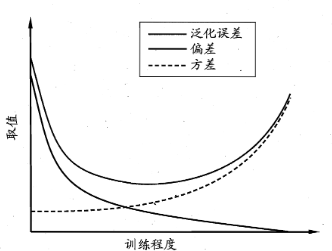
\includegraphics[width=0.309\textwidth]{pic/ML2/泛化误差与偏差, 方差的关系示意图}
    \caption{泛化误差与偏差, 方差的关系示意图}
\end{figure}

